
% --------------------------------
% studies, performance


% ==============
%
% --------------
\section{Parallel Strong Scaling and Comparison with OpenCMISS Iron}\label{sec:parallel_strong_scaling_opencmiss}

After the performance of different optimization types has been evaluated for a scenario with a single number of MPI processes in the last section, we now conduct a strong scaling study with the optimization type \code{fast-vc-apx-e}, which was found to be the most performant, and compare the runtimes to the reference software OpenCMISS Iron.

\subsection{Evaluation of Runtimes}\label{sec:strong_scaling_runtimes_opencmiss_opendihu}
For a fair comparison, we take care to exactly compute the same scenario with both software packages. The simulated scenario uses the same model as in the previous section: fiber based electrophysiology with the monodomain model given by \cref{eq:monodomain} on every muscle fiber, including the 1D electric conduction along the fibers and the 0D subcellular model of Shorten et al. \cite{Shorten2007}. The fibers are coupled with the bidomain equation in \cref{eq:bidomain1}, which is solved on the 3D domain to yield the EMG signals. No fat layer is considered in this study, as this feature is not available in our OpenCMISS implementation.

The simulated scenario contains 81 fibers with \num{1480} elements each, a coarse 3D mesh with \num{775} nodes and \num{6718591} degrees of freedom in total. 
We use our improved OpenCMISS setup, which is discussed in \cref{sec:opencmiss_numeric_improvements} and employs the second order numerical timestepping schemes and the improved linear solvers:
The monodomain model is solved using a Strang operator splitting with Crank-Nicolson and Heun's methods. A conjugate-gradient solver is used for the linear system of the bidomain equation.

We use timestep widths of $\dt_\text{0D}=\SI{1e-4}{\milli\second}$, $\dt_\text{1D}=\dt_\text{splitting}=\SI{5e-4}{\milli\second}$, $\dt_\text{3D}=\SI{1e-1}{\milli\second}$ and a simulation end time of $t_\text{end}=\SI{2}{\milli\second}$. 
During this time, the resulting values are written to output files after every $\SI{0.1}{\milli\second}$. 
The fibers are assigned to 10 MUs that are activated in a ramp every $\SI{0.2}{\milli\second}$ from $t=\SI{0}{\milli\second}$ to $t=\SI{1.8}{\milli\second}$.

Within the strong scaling study, the same scenario is computed with different numbers of processes, ranging from one to 18 in this case. We use the cubes partitioning strategies presented in \cref{sec:opencmiss_parallel_partitioning} in both OpenCMISS and OpenDiHu.
The study is executed on the same Intel Core i9-10980XE processor as the studies in the previous section.
We measure the total user time of the simulation program, which includes the runtimes for initialization, computation of system matrices and the duration of file output. However, the majority of the runtime in this scenario is spent in the numerical solvers.

In OpenDiHu, we use the setup corresponding to the \code{fast-vc-apx-e} scenario in the last section with enabled approximation of log and exp functions. We measure the runtime of two variants. The first variant computes all subcellular models and performs the same work as the OpenCMISS Iron implementation. In the second variant, the adaptive computation described in \cref{sec:adaptive_computation_for_fiber_based} is enabled, which only computes fibers that have been activated and the subcellular models that are not in equilibrium. For the chosen ramp activation pattern of the MUs, the second variant computes approximately only half of the subcellular model instances.

% weak scaling runtime
\begin{figure}
  \centering%
  \begin{subfigure}[t]{0.49\textwidth}%
    \centering%
    \includegraphics[width=\textwidth]{images/results/studies/0_strong_scaling_runtime.pdf}%
    \caption{Runtime of the simulation programs for OpenCMISS (blue) and two variants of OpenDiHu (orange and green), see the description in the text for details. 
    %For OpenDiHu, two variants are shown: the normal computation of all fibers (orange) and the optimization that computes only subcellular model instances that are not in equilibrium (green). In addition, the problem is solved on the GPU (red).
    }%
    \label{fig:0_strong_scaling_runtime}%
  \end{subfigure}
  \quad
  \begin{subfigure}[t]{0.47\textwidth}%
    \centering%
    \includegraphics[width=\textwidth]{images/results/studies/0_strong_scaling_memory.pdf}%
    \caption{Memory consumption per process at the end of the program.}%
    \label{fig:0_strong_scaling_memory}%
  \end{subfigure}   
  \caption{Electrophysiology Solver in OpenDiHu: Strong scaling study of fiber based electrophysiology and comparison between the implementations of OpenDiHu and OpenCMISS Iron. The same scenario is solved with both software packages and for increasing numbers of processes from one to 18.}%
  \label{fig:0_strong_scaling}%
\end{figure}%

\Cref{fig:0_strong_scaling_runtime} shows the resulting runtimes in this study. It can be seen that the runtime decreases monotonically for higher numbers of processes for all three tested simulations. The OpenDiHu implementation exhibits lower runtimes for all numbers of processes. The reduction in runtime between OpenCMISS Iron and the first OpenDiHu variant is given by a factor of approximately 100 with a maximum factor of 186 for 4 processes. In addition, the second OpenDiHu variant approximately halves the runtimes as expected, because only half of the subcellular models are computed.

In summary, the improvements to the EMG simulation software, which are described in this work, include the numerical improvements in \cref{sec:opencmiss_numeric_improvements} with a speedup of 2.5, the software improvements with a speedup of over 100 and a measured maximum of 186, and the algorithmic improvement of adaptive 0D model computations, whose speedup factor is scenario dependent. In the present study, the two latter factors, i.e., the speedup between the improved OpenCMISS Iron software and the OpenDiHu scenario with adaptive computation, give a combined maximum speedup of 363 for the measurement with two processes.

Moreover, the computation of this study was also carried out with the \code{gpu} optimization type in OpenDiHu, using the same GPU as in the last section. One process was started on the CPU, which offloaded the computational work of the 0D and 1D problems to the GPU. However, the GPU memory was not sufficient for the computation of all 81 fibers. Therefore, we only compute one fiber, but keep the rest of the simulation scenario equal to the other measurements. The req square in \cref{fig:0_strong_scaling_runtime} shows the measured runtime multiplied by the factor 81 for compensation. As in the studies of the previous section, the computation on the GPU has higher runtimes than the computation on the CPU.

As the memory consumption was a limiting factor for parallelism in OpenCMISS Iron as shown in \cref{sec:opencmiss_memory}, we also measure the memory consumption per process at the end of the simulation in both software frameworks. \Cref{fig:0_strong_scaling_memory} shows the result for OpenCMISS and OpenDiHu. The two variants of OpenDiHu have the same memory consumption characteristics, as the only difference between the variants is that the computation of certain subcellular models is switched on or off. 

It can be seen that the increased parallelism leads to a reduction of the used memory per process in both softwares. OpenDiHu approaches a saturation value of $\SI{200}{\mebi\byte}$ for eight and more processes. For OpenCMISS, the memory consumption is higher, but reduces more quickly also for higher numbers of processes. However, the relation between the two curves increases from a value of $\SI{6.168}{\gibi\byte} : \SI{1.078}{\gibi\byte} = 5.7$ for one process to $\SI{2.054}{\gibi\byte} : \SI{0.202}{\gibi\byte} = 10.2$ for 18 processes.

As a result, this study shows a large memory efficiency improvement in OpenDiHu compared with the OpenCMISS Iron software. For OpenCMISS, the memory scaling in this parallel strong scaling scenario is not as bad as in the parallel weak scaling considered in \cref{fig:opencmiss_memory} in \cref{sec:opencmiss_memory}. However, the total memory for all processes still increases to approximately $18 \cdot \SI{2.054}{\gibi\byte} \approx \SI{37}{\gibi\byte}$, which is higher than the main memory capacity of the used processor.

% roofline model
\begin{figure}[H]
  \centering%
  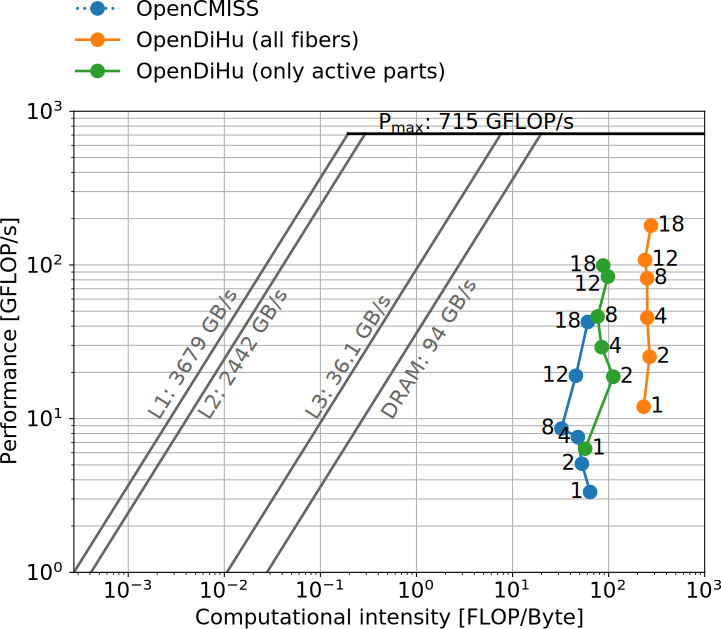
\includegraphics[width=0.8\textwidth]{images/results/studies/0_roofline.pdf}%
  \caption{Electrophysiology model in OpenDiHu: Roofline model of the strong scaling study. The blue, green and orange data points correspond to the runs of the OpenCMISS and OpenDiHu variants, as given in \cref{fig:0_strong_scaling_runtime}.}%
  \label{fig:0_roofline}%
\end{figure}%

\subsection{Roofline Model}\label{sec:roofline_model}
To further investigate the computational behavior, we also present the performance measurements of the solvers in a roofline model. 
\Cref{fig:0_roofline} shows the resulting diagram with the data points of all CPU runs in the strong scaling study of \cref{fig:0_strong_scaling_runtime}. The $x$ axis shows the computational intensity of the simulation, which is measured in double-precision floating-point operations (FLOP) per byte of data that are transferred between the CPU and the main memory and caches. The $y$ axis measures the performance in GFLOPs per second. The highest possible performance is given by the peak performance of the processor, which is $P_\text{max} = \SI{715}{\giga\flop\per\second}$ in this case. Furthermore, the performance is limited by the amount of payload data that can be transferred to the CPU over the memory bus. The memory bandwidths of the L1, L2 and L3 caches and the main memory (DRAM) correspond to the shown diagonals in \cref{fig:0_roofline} and form the \say{roofline} of the model.

We measured the memory bandwidths of the Caches and the peak performance using the Empirical Roofline Tool \cite{ert}. The main memory bandwidth was retrieved from the processors' documentation.

To locate the simulation runs of the study in the roofline model, we used hardware counters to count floating point instructions and memory access operations.
For the runs with OpenCMISS Iron and OpenDiHu, we started the hardware counters \SI{90}{\second}, respectively \SI{15}{\second} after the beginning of the simulation, such that the initialization phase was not included in the measured data. The counters were kept active for 15, 30 and 60 seconds, depending on the expected runtimes of the different runs. The counted numbers of events were then divided by the acquisition time to yield the required rates of memory bandwith and floating-point performance.

\Cref{fig:0_roofline} shows the measured points in the roofline model corresponding to the curves in \cref{fig:0_strong_scaling_runtime}. All data points are located at the right hand side of the memory bandwidth limits, which indicates that the simulation is compute bound. 
The highest computational intensity and performance are both achieved by the OpenDiHu variant given in orange color, which computes all fibers and subcellular models regardless of their activation state. The values for the adaptive variant given in green color are lower, as less computations are performed and a higher portion of the runtime and compute power is spent on determining which subcellular model has to be computed. The two metrics are lowest for the OpenCMISS runs given in blue color.

The roofline diagram shows the data points for all parallel runs and the number of processes is noted in the plot. The run with 18 processes is the most meaningful, as this means that the whole processor is employed. The largest performance for the OpenDiHu run in orange color has a value of \SI{180.157}{\giga\flop\per\second} which corresponds to \SI{25.2}{\percent} of the peak performance and is a very good value. The rated \SI{100}{\percent} of peak performance for processors are practically unreachable. For example, the peak performance assumes only fused multiply add operations and requires a power management that maximizes the employment of the boost clock frequency in the processor. These conditions are not fulfilled in our computations of realistic models and scenarios.
The performance values of the runs with 18 processes for the green and blue data points are \SI{13.9}{\percent} and \SI{6.0}{\percent}, respectively. 

Furthermore, the measurements with lower process counts can also be assessed with a scaled down peak performance according to the fraction of used cores. However, this assessment is slightly off, as, e.g., the CPU can use a higher clock frequency, if only the heat dissipation of one active core has to be compensated. The performance for the OpenDiHu run with one process given by the orange point is \SI{11.966}{\giga\flop\per\second}, which corresponds to \SI{30.1}{\percent} of the fractional peak performance of $\SI{715}{\giga\flop\per\second}/18 = \SI{39.7}{\giga\flop\per\second}$.

% Crank-Nicolson
% scenario_name: vc-1-ws,  n_subdomains: 1 1 1,  n_ranks: 1,  end_time: 2.0 
% dt_0D:           1e-04, diffusion_solver_type:      cg  
% dt_1D:           5e-04, potential_flow_solver_type: gmres, approx. exp.: True
% dt_splitting:    5e-04, emg_solver_type:            cg, emg_initial_guess_nonzero: False
% dt_3D:           1e-01, paraview_output: True, optimization_type: vc, enable_weak_scaling: True
% output_timestep: 1e-01  stimulation_frequency: 1.0 1/ms = 1000.0 Hz
% fiber_file:              /data/scratch/maierbn/opendihu/examples/electrophysiology/input/left_biceps_brachii_9x9fibers.bin
% cellml_file:             /data/scratch/maierbn/opendihu/examples/electrophysiology/input/new_slow_TK_2014_12_08.cellml
% fiber_distribution_file: /data/scratch/maierbn/opendihu/examples/electrophysiology/input/MU_fibre_distribution_10MUs.txt
% firing_times_file:       /data/scratch/maierbn/opendihu/examples/electrophysiology/input/MU_firing_times_immediately.txt
% ********************************************************************************
% prefactor: sigma_eff/(Am*Cm) = 0.03079310344827586 = 8.93 / (500.0*0.58)
% diffusion solver type: cg
% n fibers:              81 (9 x 9)
% n points per fiber:    1481
% 1 rank, partitioning: x1 x y1 x z1
% 9 x 9 = 81 fibers, per partition: 9 x 9 = 81
% per fiber: 1D mesh    nodes global: 1481, local: 1481
%   sampling 3D mesh with stride 2 x 2 x 50  
%     linear 3D mesh    nodes global: 5 x 5 x 31 = 775, local: 5 x 5 x 31 = 775 
%     linear 3D mesh elements global: 4 x 4 x 30 = 480, local: 4 x 4 x 30 = 480 
% number of degrees of freedom:
%                     1D fiber:       1481  (per process: 1481)
%             0D-1D monodomain:      82936  (per process: 82936)
%  all fibers 0D-1D monodomain:    6717816  (per process: 6717816)
%                  3D bidomain:        775  (per process: 775)
%                        total:    6718591  (per process: 6718591)
% 

% weak scaling data
% opencmiss
% 1: duration 82046.0 s, memory consumption per process (high watermark): 6.168 GB
% 2: duration 52877.0 s, memory consumption per process (high watermark): 5.257 GB
% 4: duration 33802.0 s, memory consumption per process (high watermark): 4.639 GB
% 8: duration 17230.0 s, memory consumption per process (high watermark): 4.027 GB
% 12: duration 8840.0 s, memory consumption per process (high watermark): 2.829 GB
% 18: duration 5122.0 s, memory consumption per process (high watermark): 2.054 GB
% 
% opendihu (all fibers)
% 1: duration: 586.3s, 584.7s, memory consumption per process (high watermark): 1.078 GB, speedup to opencmiss: 139.93621121932085
% 2: duration: 303.9s, 298.9s, memory consumption per process (high watermark): 0.783 GB, speedup to opencmiss: 174.00046069301393
% 4: duration: 181.6s, 175.5s, memory consumption per process (high watermark): 0.447 GB, speedup to opencmiss: 186.09081024539964
% 8: duration: 111.9s, 104.8s, memory consumption per process (high watermark): 0.278 GB, speedup to opencmiss: 153.99740805291145
% 12: duration: 87.5s, 79.9s, memory consumption per process (high watermark): 0.249 GB, speedup to opencmiss: 100.99490645975152
% 18: duration: 58.3s, 49.7s, memory consumption per process (high watermark): 0.202 GB, speedup to opencmiss: 87.8207692747328
% 
% opendihu (only active parts)
% 1: duration: 270.1s, 268.4s, memory consumption per process (high watermark): 1.079 GB, speedup to opencmiss: 303.70534888025173
% 2: duration: 145.3s, 140.3s, memory consumption per process (high watermark): 0.783 GB, speedup to opencmiss: 363.96613436123346
% 4: duration: 96.5s, 90.3s, memory consumption per process (high watermark): 0.449 GB, speedup to opencmiss: 350.15279432330243
% 8: duration: 64.6s, 57.7s, memory consumption per process (high watermark): 0.278 GB, speedup to opencmiss: 266.7389116804706
% 12: duration: 49.4s, 41.7s, memory consumption per process (high watermark): 0.249 GB, speedup to opencmiss: 178.76944336776825
% 18: duration: 42.0s, 33.7s, memory consumption per process (high watermark): 0.202 GB, speedup to opencmiss: 122.07995127183165
% 
% roofline data:
% opencmiss
% 1 rank(s), performance: 3.332 GFLOP/s, mem bandwidth: 3.117 GB/s, intensity: 64.143 FLOP/B
% 2 rank(s), performance: 5.087 GFLOP/s, mem bandwidth: 5.793 GB/s, intensity: 52.702 FLOP/B
% 4 rank(s), performance: 7.583 GFLOP/s, mem bandwidth: 9.507 GB/s, intensity: 47.871 FLOP/B
% 8 rank(s), performance: 8.616 GFLOP/s, mem bandwidth: 16.026 GB/s, intensity: 32.276 FLOP/B
% 12 rank(s), performance: 19.012 GFLOP/s, mem bandwidth: 25.037 GB/s, intensity: 45.634 FLOP/B
% 18 rank(s), performance: 42.582 GFLOP/s, mem bandwidth: 42.175 GB/s, intensity: 60.725 FLOP/B
% 
% opendihu (all fibers)
% 1 rank(s), performance: 11.966 GFLOP/s, mem bandwidth: 1.550 GB/s, intensity: 231.674 FLOP/B
% 2 rank(s), performance: 25.273 GFLOP/s, mem bandwidth: 2.839 GB/s, intensity: 267.084 FLOP/B
% 4 rank(s), performance: 45.371 GFLOP/s, mem bandwidth: 5.396 GB/s, intensity: 252.419 FLOP/B
% 8 rank(s), performance: 81.855 GFLOP/s, mem bandwidth: 9.770 GB/s, intensity: 251.630 FLOP/B
% 12 rank(s), performance: 107.793 GFLOP/s, mem bandwidth: 13.531 GB/s, intensity: 239.385 FLOP/B
% 18 rank(s), performance: 180.157 GFLOP/s, mem bandwidth: 19.612 GB/s, intensity: 276.235 FLOP/B
% 
% opendihu (only active parts)
% 1 rank(s), performance: 6.376 GFLOP/s, mem bandwidth: 1.679 GB/s, intensity: 56.978 FLOP/B
% 2 rank(s), performance: 18.736 GFLOP/s, mem bandwidth: 2.512 GB/s, intensity: 111.957 FLOP/B
% 4 rank(s), performance: 29.185 GFLOP/s, mem bandwidth: 5.178 GB/s, intensity: 84.649 FLOP/B
% 8 rank(s), performance: 46.207 GFLOP/s, mem bandwidth: 9.046 GB/s, intensity: 76.793 FLOP/B
% 12 rank(s), performance: 84.096 GFLOP/s, mem bandwidth: 12.867 GB/s, intensity: 98.369 FLOP/B
% 18 rank(s), performance: 99.256 GFLOP/s, mem bandwidth: 17.020 GB/s, intensity: 87.893 FLOP/B



\begin{reproduce_no_break}
  The scripts to run the studies in this scenario and to create the plots are available in the repository at \href{https://github.com/dihu-stuttgart/performance}{github.com/dihu-stuttgart/performance}
  in the directory \code{opendihu/20_fibers_emg_avx_opencmiss}:
  \begin{lstlisting}[columns=fullflexible,breaklines=true,postbreak=\mbox{\textcolor{gray}{$\hookrightarrow$}\space}]
    ./0_run.sh
  \end{lstlisting}
  The directory also contains a script that performs all steps to install OpenCMISS, if needed. 
  
  Note, the studies in the previous and the current sections were carried out on the computer with hostname \code{pcsgs05} in the institute network at the time of writing.
\end{reproduce_no_break}



%-----
\section{Performance Measurements on the GPU}\label{sec:performance_gpu}

In the previous two sections, measurements were made on a GPU, which produced worse results than the CPU code. The used GPU was an NVIDIA GeForce RTX 3080, a high-end consumer graphics card, which mainly targets graphics rendering perfomance using single-precision operations. The ratio between double-precision and single-precision performance is 1:64. However, single-precision calculations were found to not yield a stable subcellular model solver, as the precision is too low. 
% quadro: https://www.techpowerup.com/gpu-specs/quadro-gp100.c2994
% RTX: https://www.techpowerup.com/gpu-specs/geforce-rtx-3080.c3621

In this section, we conduct two studies, where the first study uses the same GPU hardware as before. The second study is executed on an NVIDIA Quadro GP100 GPU, which has a double-precision to single-precision performance ratio of 1:2.
The rated double-precision performance of the Quadro card is \SI{5.168}{\tera\flops}, which is ten times higher than the value of \SI{465.1}{\giga\flops} for the GeForce card. 

The CPU hardware connected with the Quadro card contains a dual-socket CPU with two 12-core Intel Xeon Silver 4116 processors with \SI{2.1}{\giga\hertz} base frequency and \SI{3}{\giga\hertz} maximum turbo frequency, yielding a total core count of 24, and being equipped with main memory of \SI{188}{\gibi\byte}. 

Computational hardware can be compared by its average thermal design power dissipation (TDP). For the studies in the previous two sections, the TDP values for the used CPU and GPU were \SI{165}{\watt} and \SI{320}{\watt}. For the second study in the current section, the values for CPU and GPU are $2\cdot \SI{85}{\watt} = \SI{170}{\watt}$ and \SI{235}{\watt}. This indicates that the employed hardware is in a comparable electrical power range. However, the GPU is more specialized for our double-precision needs.

\subsection{Strong Scaling with the GPU for the Hodgkin-Huxley Model}\label{sec:strong_scaling_gpu_hodgkin_huxley}

While the studies in the last two sections only used one process on the CPU, which managed the offloaded computations on the GPU,
we now additionally consider parallelism on the CPU.

The first study compares the strong scaling with and without GPU acceleration. The runs with GPU acceleration partition the computational domain as usual to multiple subdomains, which are handled by dedicated processes on the CPU. The solution of the 0D and 1D models is performed on the GPU, and every process independently transfers its part of the computational work to the same GPU. The 3D model is fully solved using MPI parallelism on the CPU. We compare this setup with a pure CPU based strong scaling study.

The scenario solves the fiber based electrophysiology model without fat layer with 169 fiber meshes of 1480 elements each and a 3D mesh with 1984 elements. The subcellular model of Hodgkin and Huxley \cite{Hodgkin1952} is used. The computation uses the same numerical parameters as in the first study in \cref{sec:evaluation_of_code_gen}, a 3D solver timestep of $\dt_\text{3D}=\SI{4e-01}{\ms}$ and a simulation end time of $\SI{10}{\ms}$. Moreover, the setup equals the settings of the \code{fast-vc} and \code{fast-gpu} scenarios in \cref{sec:evaluation_of_code_gen}.

\begin{figure}%
  \centering%
  \begin{subfigure}[t]{0.45\textwidth}%
    \centering%
    \includegraphics[height=52mm]{images/results/studies/16_hodgkin_huxley_gpu.pdf}%
    \caption{Study, where every process on the CPU offloads the 0D and 1D model computations to the GPU.}%
    \label{fig:16_hodgkin_huxley_gpu}%
  \end{subfigure}
  \,
  \begin{subfigure}[t]{0.53\textwidth}%
    \centering%
    \includegraphics[height=52mm]{images/results/studies/16_hodgkin_huxley_cpu.pdf}%
    \caption{CPU-only study.}%
    \label{fig:16_hodgkin_huxley_cpu}%
  \end{subfigure}   
  \caption{Electrophysiology model in OpenDiHu: Strong scaling study with and without GPU usage. A scenario with 169 fibers and the subcellular model of Hodgkin and Huxley is simulated. The vertical bars indicate the standard deviation of the runtimes in the set of measurements, which consists of multiple runs and the values of all processors in every run.}%
  \label{fig:16_hodgkin_huxley_cpu_gpu}%
\end{figure}%

\Cref{fig:16_hodgkin_huxley_cpu_gpu} presents the results for the two studies with and without GPU usage. \Cref{fig:16_hodgkin_huxley_cpu} shows the runtimes of different parts in the simulation of the CPU-only strong scaling study. It can be seen that the 0D computations account for most of the runtime, followed by the 1D computations. The 0D computations involve the solution of the Hodgkin-Huxley subcellular model. The 1D computations consists of solving 1D problems in serial using the Thomas algorithm. The 3D solver time is negligible as the 3D problem is only solved every \num{13333} timesteps. The 3D solution is only required right before the VTK file output step for the EMG values. This step occurs every $\SI{0.4}{\ms}$, which corresponds to an EMG sampling frequency of \SI{2.5}{\kilo\hertz}.
The runtimes for initialization and the file output itself are also very low compared with the runtimes of the computations.

\Cref{fig:16_hodgkin_huxley_cpu} shows that the total runtime decreases with higher process counts in this strong scaling study. The parallel efficiency $E_p = T_1/(T_p\,p)$ reaches $E_p=\SI{65.2}{\percent}$ for $p=18$ processes. We observe that the 0D and the 1D solver and the VTK file output have good strong scaling properties, whereas the initialization and the solution of the 3D model contain serial code portions that prohibit optimal scaling.

\Cref{fig:16_hodgkin_huxley_gpu} shows the analog study, where the 0D and 1D computations are offloaded to the GPU. The runtimes of these individual model parts are not explicitely measured, only the total runtime is known.

The plot shows an increasing total runtime for higher CPU parallelism. 
The runtimes for initialization, file output and the 3D solver are equal to the CPU-only study.
The increasing total runtime shows that the GPU is better at solving the complete 0D and 1D problems 
given by one CPU process than at the same computation, but split to several parts and provided by different MPI processes. 
The benefit of using multiple CPU processes to interface the GPU in this study is, thus, only that the VTK output functionality gets parallelized. However, this effect is negligible.

An absolute comparison between the runtimes in \cref{fig:16_hodgkin_huxley_gpu} and \cref{fig:16_hodgkin_huxley_cpu} also reveals that the scenarios for one to 18 processes using the GPU have 4.8 to 181 times longer total runtimes. In this study, the memory transfer between the CPU and the GPU has a low influence on the total runtime, as this transfer only happens before and after the 3D model is solved. The measured runtimes, therefore, correspond to the computation on the GPU.

%0/18 : This is opendihu 1.2, built Jan 16 2021, C++ 201402, GCC 10.2.0, current time: 2021/1/17 12:37:12, hostname: pcsgs02, n ranks: 18
%0/18 : Open MPI v3.1.6, package: Open MPI maierbn@sgscl1 Distribution, ident: 3.1.6, repo rev: v3.1.6, Mar 18, 2020
%0/18 : File "/data/scratch/maierbn/opendihu/examples/electrophysiology/fibers/fibers_emg/settings_fibers_emg.py" loaded.
%0/18 : ---------------------------------------- begin python output ----------------------------------------
%Loading variables from "/data/scratch/maierbn/performance/opendihu/16_hodgkin_huxley_gpu/hodgkin_huxley_gpu.py".
%scenario_name: gpu-18,  n_subdomains: 3 2 3,  n_ranks: 18,  end_time: 10.0
%dt_0D:           3e-05, diffusion_solver_type:      cg
%dt_1D:           1e-05, potential_flow_solver_type: gmres
%dt_splitting:    3e-05, emg_solver_type:            cg, emg_initial_guess_nonzero: False
%dt_3D:           4e-01, paraview_output: True, optimization_type: gpu, use_single_precision: False
%output_timestep: 4e-01  stimulation_frequency: 0.1 1/ms = 100.0 Hz
%fiber_file:              /data/scratch/maierbn/opendihu/examples/electrophysiology/input/left_biceps_brachii_13x13fibers.bin
%cellml_file:             /data/scratch/maierbn/opendihu/examples/electrophysiology/input/hodgkin_huxley_1952.c
%fiber_distribution_file: /data/scratch/maierbn/opendihu/examples/electrophysiology/input/MU_fibre_distribution_10MUs.txt
%firing_times_file:       /data/scratch/maierbn/opendihu/examples/electrophysiology/input/MU_firing_times_always.txt
%********************************************************************************
%prefactor: sigma_eff/(Am*Cm) = 0.03079310344827586 = 8.93 / (500.0*0.58)
%diffusion solver type: cg
%n fibers:              169 (13 x 13)
%n points per fiber:    1481
%18 ranks, partitioning: x3 x y2 x z3
%13 x 13 = 169 fibers, per partition: 4 x 6 = 24
%per fiber: 1D mesh    nodes global: 1481, local: 494
  %sampling 3D mesh with stride 2 x 2 x 50 
    %linear 3D mesh    nodes global: 8 x 8 x 31 = 1984, local: 3 x 4 x 10 = 120
    %linear 3D mesh elements global: 7 x 7 x 30 = 1470, local: 3 x 4 x 10 = 120
%number of degrees of freedom:
                    %1D fiber:       1481  (per process: 494)
            %0D-1D monodomain:       5924  (per process: 1976)
 %all fibers 0D-1D monodomain:    1001156  (per process: 47424)
                 %3D bidomain:       1984  (per process: 120)
                       %total:    1003140  (per process: 47544)
%Python config parsed in 0.1s.

\subsection{Evaluation of Hybrid CPU and GPU Computation for the Shorten Model}\label{sec:evaluation_hybrid}

Whereas previously, the subcellular model of Hodgkin and Huxley was solved on the GPU, we now switch to the more compute intense model of Shorten et al. \cite{Shorten2007}. This model has higher memory demands, such that it is not possible to solve it with OpenMP 4.5 for a muscle fiber mesh with 1481 nodes on the GeForce RTX 3080 GPU. As noted before, we use the NVIDIA Quadro GP100 GPU for the next study.
This GPU is also not capable of solving the whole set of 1481 models instances per fiber for 169 fibers at the same time. For one instance of the subcellular model, 57 state and rate variables each, and 71 intermediate variables have to be stored, along with other data, such as element lengths for every element.

Thus, we follow a hybrid approach. We parallelize the scenario to 27 processes on the CPU. Only one process offloads its subdomain to the GPU. In this way, both the CPU and the GPU take part in the computation and the available hardware capabilities are fully exploited.

\begin{figure}
  \centering%
  \includegraphics[width=0.9\textwidth]{images/results/studies/gpu_parallelization.png}%
  \caption{Electrophysiology solver in OpenDiHu: Partitioning of the 169 fibers to 27 processes used in the runtime study with hybrid CPU-GPU usage. The image also shows the resulting EMG signals $\phi_e$ on the muscle surface.}%
  \label{fig:gpu_parallelization}%
\end{figure}

The scenario and the numerical parameters are the same as described for the study with the Shorten model in \cref{sec:evaluation_of_code_gen}. 49 muscle fibers are used and parallelized to $3\times 3\times 3=27$ subdomains. \Cref{fig:gpu_parallelization} visualizes the partitioning of the fibers by different colors and the EMG values $\phi_e$ on the muscle surface at the simulation end time of $t_\text{end}=\SI{10}{\ms}$.

\Cref{fig:17_shorten_gpu} visualizes the runtimes of two runs. The first bar only employs the CPU and provides the reference for the measured runtimes. The second bar corresponds to the hybrid run, where one process employs the GPU. The 0D and 1D solver runtimes in the second bar are averaged over the CPU computations. The total runtime involves both the CPU and the GPU computations.
It can be seen that the total runtime given by the total bar heights is higher for the hybrid run. In the hybrid runs, the CPU processes have to wait at the synchronization point in the solution of the 3D problem until the GPU process has completed the 0D/1D computations.

\begin{figure}
  \centering%
  \includegraphics[width=0.6\textwidth]{images/results/studies/17_shorten_gpu.pdf}%
  \caption{Electrophysiology model in OpenDiHu: Runtime study for a CPU-only computation and a hybrid parallelization that employs both the CPU and the GPU. For the hybrid approach, one of the 27 partitions was computed on the GPU. The compute-intense subcellular model of Shorten et al. is simulated.}%
  \label{fig:17_shorten_gpu}%
\end{figure}

\subsection{Conclusion}

Several scenarios with computations of the 0D subcellular and 1D electric conduction models on the GPU have been evaluated. 
\Cref{sec:evaluation_of_code_gen} compared the runtime for the Hodgkin-Huxley subcellular model on 625 fibers on the GPU with implementations on the CPU.
In \cref{sec:strong_scaling_runtimes_opencmiss_opendihu}, the computation on the GPU with the Shorten subcellular model was measured for one fiber.
\Cref{sec:strong_scaling_gpu_hodgkin_huxley} conducted a strong scaling study with the Hodgkin-Huxley model on 169 fibers and \cref{sec:evaluation_hybrid} evaluated a hyprid approach, where the Shorten model on different fibers was computed on the GPU and the CPU at the same time. This last study used a GPU with higher double-precision performance than the previous studies.

In all of these studies, the GPU computations could not compete with their CPU counterparts. The GPU implementation of the models relied on target-specific CUDA code, which was automatically generated by the OpenMP 4.5 pragmas produced by the code generator in OpenDiHu. The CPU computations used highly optimized CPU code with explicit vector instructions, an approach that is close to optimal as shown by the roofline model in \cref{sec:roofline_model}. Thus, the comparison considers different levels of optimization. We cannot conclude in general that the GPU is less suited to solve the the fiber based electrophysiology models than the CPU. However, the GPU support in OpenMP is not competitive with our optimized CPU implementation.

The required GPU support of OpenMP in the GNU compiler is functional to the extend needed in our studies only since GCC version 11, which, at the time of writing, is still experimental and not yet released. Further performance gains can be expected in the future as compiler development advances. One problem is also the high memory requirement for the subcellular models, which only allows a certain number of subcellular model instances to be computed on the given hardware. It is also not clear, whether the high memory consumption is also an artifact of the compiler and will reduce with later compiler versions.

Despite the lower performance, it was shown that OpenDiHu can be used to solve the monodomain equation \cref{eq:monodomain} with different subcellular models on the GPU. Switching between the CPU and GPU variants can be accomplished by only changing the \code{optimizationType} parameter between \code{`vc`} and \code{`gpu`}. Hybrid strategies, where some processes use \code{`vc`} and others \code{`gpu`}, have been demonstated.

In future work, the performance issue of the GPU computations can be addressed by using different technologies to access the compute power of GPUs.
Examples are to directly use the CUDA programming language or the C++ based abstraction layer for acceleration hardware SYCL \cite{sycl}. OpenDiHu already provides a reference implementation for such improvements by the code generator, which outputs model specific code with OpenMP pragmas for GPU offloading. This code implements proper, economical data transfer between the devices and contains hints how to distribute the workload on the GPU by the respective pragma placements. It could be used as a starting point to integrate further \say{optimization types} in the code generator.

%-----

% GPU slower in all studies
% comparison with highly optimized CPU code, near optimal
% GPU OpenMP not yet optimal, requires experimental GCC 11
% problem is also memory requiremnet
% GPU can be easily switched, hybrid is possible in opendihu
% future work: SYCL, CUDA extended code generator


\begin{reproduce_no_break}
  The scripts to run the studies and to create the plots for \cref{fig:16_hodgkin_huxley_cpu_gpu,fig:17_shorten_gpu} are available in the repository at \href{https://github.com/dihu-stuttgart/performance}{github.com/dihu-stuttgart/performance}
  in the directories \code{opendihu/16_hodgkin_huxley_gpu} and  \code{opendihu/17_shorten_gpu}.
\end{reproduce_no_break}


% ------------
%
% f===========
